%%%%%%%%%%%%%%%%%%%%%%%%%%%%%%%%%%%%%%%%%%%%%%%%%%%%%%%%%%%%%%%%%%%%%%%%
%                                                                      %
%     File: Thesis_Results.tex                                         %
%     Tex Master: Thesis.tex                                           %
%                                                                      %
%     Author: Andre C. Marta                                           %
%     Last modified :  2 Jul 2015                                      %
%                                                                      %
%%%%%%%%%%%%%%%%%%%%%%%%%%%%%%%%%%%%%%%%%%%%%%%%%%%%%%%%%%%%%%%%%%%%%%%%



\chapter{DVFS Application to Deep Learning}
\label{chapter:application}

From the set of applications that are known to be imprecision tolerant, deep learning stands out as one of the most prominent ones. This chapter starts by providing an overview of what is a deep learning application. It is followed by a characterization of the type of benchmarks that will be used along the development of the proposed work. The final section introduces some preliminary results demonstrating that voltage and frequency exploration outside the conventional DVFS limits can benefit deep learning applications execution, focusing on energy consumption optimization.

\section{Deep Learning Overview}
\label{sec:DLO}
Deep Learning (DL) is a subset of the larger family of Machine Learning methods. Also known as deep structured learning or hierarchical learning, this type of algorithms is based on artificial neural networks and can be utilized for supervised, semi-supervised, and unsupervised learning \cite{bengio_representation_2013} \cite{schmidhuber_deep_2015}.

Biological systems inspired the creation of Artificial Neural Networks (ANN), in which Deep Learning architectures are built on top. This information-processing and distributed communications type of network operates by mimicking a simplistic biological brain, where the interconnection between the neurons is static and symbolic \cite{marblestone_toward_2016}. 

Different deep learning architectures are being developed, such as convolutional neural networks (CNN), recurrent neural networks (RNN), and unsupervised pre-trained networks (UPT). These have been applied to a diversity of fields, including computer vision, speech and audio recognition, natural language processing, bioinformatics, and others. In such applications, deep learning algorithms are being able to achieve comparable and, in some cases, superior results to humans experts \cite{noauthor_googles_nodate}.

\begin{figure}[!htb]
  \centering
  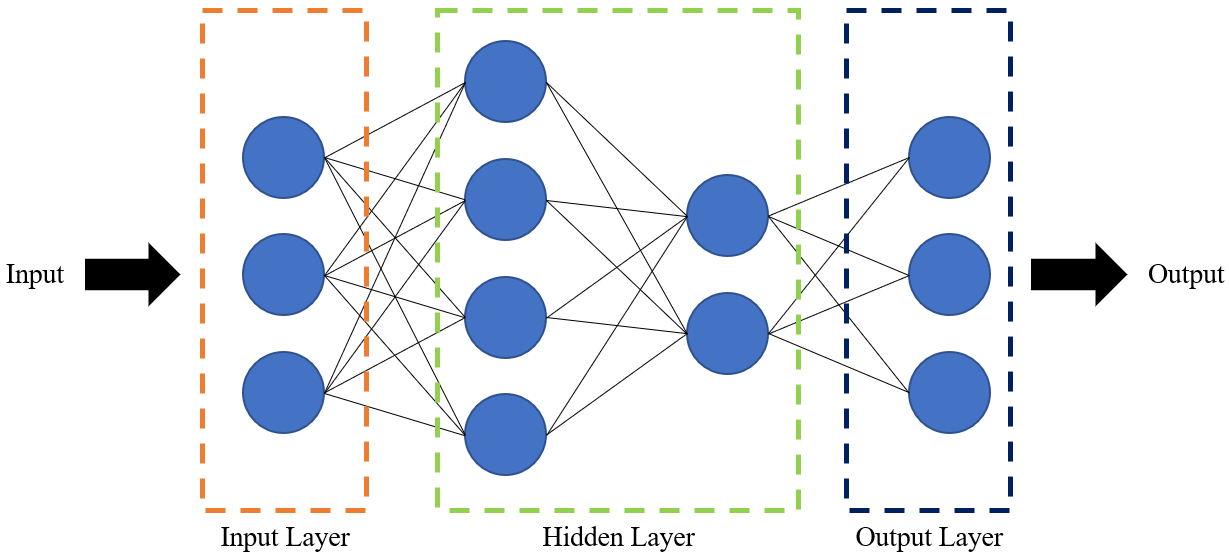
\includegraphics[width=0.75\textwidth]{Figures/DL/DNNarch.png}
  \caption[]{Model of fully-connected (feedforward) network.}
  \label{fig:DNNarch}
\end{figure}


\subsection{Deep Neural Network}
The unitary element of a deep neural network (DNN) is the artificial neuron. This element can be mathematically modeled by a set of multiplications and summations, as shown in Equation \ref{eq:neuron}, where $W_i$ represents the weight and $b$ the bias applied on each artificial neuron.

\begin{equation}
\label{eq:neuron}
    Y = \sum_{i=1}^{n} W_iX_i+b
\end{equation}

One of the significant benefits of deep neural networks is their ability to capture none linear relationships between the input parameters. For such purpose, an activation function is attached to each neuron, helping him to handle scenarios where problems are not linearly separated \cite{dong_dnnmark:_2017}. The most common non-linear activation functions are  hyperbolic tangent (tanh) \cite{orr_neural_1998}, Rectified Linear Unit (ReLU) \cite{orr_neural_1998} and sigmoid \cite{orr_neural_1998}. The architecture of the deep neural network is the combination of the linear transformations performed by the neurons plus the non-linear activation functions.

A neural network is composed of arrangements of neurons and activation functions in layers. Each layer is responsible for applying a series of transformations to the data accordingly to the weight and bias value stored in each artificial neuron. A deep neural network is composed of at least three layers, the input layer, with a number of neurons equal to the input size, at least one hidden layer, being this the distinguishing characteristics of a DNN, and an output layer with the number of neurons equal to the output size. The different organization of the layers in number size, type of operation and number of connections of layers defines the type and architecture of the DNN.

\subsection{Training and Inference}
The mathematical description of the DNN training process, (see Equation \ref{eq:loss}), is equivalent to treating the network as a loss function $L$, where inputs $X$, outputs $Y$ and the network's parameters weights - $W$ and bias $b$ are function arguments. The objective of the training session is to optimize the in-network parameters of $W$ and $b$ to minimize the overall loss.

\begin{equation}
    \label{eq:loss}
    (W,b) = \arg\min_{W} L(X,Y,W,b)
\end{equation}

The DNN training is an iterative process, where at the end of each iteration, a loss value is computed, and the set of in-network parameters is updated. This loss value represents how well are the input parameters being modeled by the network. As the number of training iterations increase, the loss value reduces and converges to a minimum, at which the model accuracy prediction will be at its maximum. At this point, the training session can be stopped.

The most common method for the parameters update is the Stochastic Gradient Descent (SGD) algorithm, (see Equation \ref{eq:update}), an iterative algorithm that, after processing mini-batches of the training data, computes new weights and bias for each neuron. 

\begin{equation}
    \label{eq:update}
    W_{i+1} \xleftarrow{} W_i - \alpha \sum_{n=1}^{m}\frac{\partial L}{\partial W_i}
\end{equation}

In Equation \ref{eq:update}, $m$ represents the number of mini-batches to run, $W_i$ is the current parameter, $W_{i+1}$ the update parameter, $\alpha$ the learning rate and $\frac{\partial L}{\partial W_i}$ the partial derivative of the loss function $L$ in order to the parameters. This last equation is obtained by applying the derivative chain rule in a backward-cascade fashion with respect to inputs, outputs, and parameters of each DNN layer.

Each iteration of the training process is composed of forward and backward propagation. On the forward propagation, the loss function for the current in-network parameters is evaluated, computing the loss value. By performing the backward propagation, the partial derivative $\frac{\partial L}{\partial W_i}$ of each of the parameters is obtained to apply the SGD algorithm. 

The inference (or prediction) process corresponds to performing a forward propagation, with the intended inputs, on a previously trained neural network. At the output layer, a set of values (or probabilities) are computed, corresponding to the prediction that the model gave to the given inputs.

\section{Benchmarks}

For the definition of the novel DVFS aware mechanism, three types of benchmarking applications are going to be needed. In the first stage, the characterization of non-conventional DVFS parameters starts by analyzing simple kernels, where different parts of the GPU architecture are stressed, and the effects of combine work types are tested. On the second stage, The simple GPU kernels are combined, forming abstract and independent kernels that represent the variety of work that is performed on the many layer types that compose a DNN model. The last benchmarks, where the complete DVFS aware mechanism is tested, are the fully-fledged state of the art deep neural networks models used nowadays in the use cases stated at Section \ref{sec:DLO}.

\subsection{Fundamental Analysis}
\label{sec:funAnal}

The fundamental analysis and characterization of the GPU are done by running and profiling simple benchmarks that stress the different components of the GPU architecture. Following the same strategy used by Guerreiro \textit{et al.} in \cite{guerreiro_gpgpu_2018} \cite{guerreiro_modeling_2019}, a set of benchmarks are devised that fit inside of six categories: arithmetic, special units, branch, shared memory, L2 cache and DRAM.  Listings 3.1 to 3.6 exemplify the skeleton of each category of benchmarks.

Listing 3.1 exercises the arithmetic part of the CU, by performing sequences of multiplications and sums, with data presented on each CU registers. By changing the DATA\_TYPE parameter between int,  float and double, the effects of the type of operand and increased precision can be studied. The benchmark execution starts by each thread loading a value from the global memory to its registers. It is followed by a variable sequence of size \textit{N} of arithmetic operations followed by placing the computed value back on the global memory. By varying \textit{N}, it can be studied the data utilization rate (number of instructions performed to each pair of load/store instructions).


Listing 3.2 exercises special arithmetic units devised to compute non-linear functions (as the ones used by deep learning applications). Similarly to Listing 3.1, this benchmark starts by loading a value from the global memory, then performs a sequence of size \textit{N} of arithmetic operations and it ends by storing the value back on the global memory.

\noindent\begin{minipage}{.45\textwidth}[!b]
\centering
\begin{lstlisting}[language=C, caption={Int, SP, DP Code}]
DATA_TYPE r0, r1, r2, r3;

r0=A[threadId]; 
r1=r2=r3=r0; 
for (int i=0;i<N;i++) { 
    r0 = r0 * r0 + r1;  
    r1 = r1 * r1 + r2; 
    r2 = r2 * r2 + r3;  
    r3 = r3 * r3 + r0; 
} 
B[threadId]=r0;
\end{lstlisting}
\end{minipage}\hfill
\begin{minipage}{.45\textwidth}
\centering
\begin{lstlisting}[language=C, caption={SF Code}]
DATA_TYPE r0, r1, r2, r3;

r0=A[threadId]; 
r1=r2=r3=r0; 
for(int i=0;i<N;i++) {  
    r0 = log(r1);  
    r1 = cos(r2);  
    r2 = log(r3);  
    r3 = sin(r0);
} 
B[threadId]=r0;
\end{lstlisting}
\end{minipage}
\noindent\begin{minipage}{.38\textwidth}[!b]
\centering
\begin{lstlisting}[language=C, caption={Branches Code}]
DATA_TYPE r0, r1, r2, r3;

r0=A[threadId]; 
r1=r2=r3=r0; 
for(int i=0;i<N;i++) {  
    r0 = r0 * r0 + r1;  
    if( r0 > 0)
        r1 = r1 * r1 + r2; 
    else 
        r1 = r3 * r3 - r2; 
    r0 = r3 * r3 + r0; 
} 
B[threadId]=r0;
\end{lstlisting}
\end{minipage}\hfill
\begin{minipage}{.59\textwidth}
\centering
\begin{lstlisting}[language=C, caption={Shared Memory Code}]
__shared__ DATA_TYPE shared[THREADS]; 
DATA_TYPE r0; 

for(int i=0;i<COMP_ITERATIONS;i++) {  
    r0 = shared[threadId];      
    shared[THREADS - threadId - 1] = r0;
}
\end{lstlisting}
\end{minipage}
\noindent\begin{minipage}{.55\textwidth}[!b]
\centering
\begin{lstlisting}[language=C, caption={L2 Cache Code}]
DATA_TYPE r0;

for(int i=0;i<COMP_ITERATIONS;i++) {      
    r0 = cdin[threadId];      
    cdout[threadId]=r0;
} 

cdout[threadId]=r0;
\end{lstlisting}
\end{minipage}\hfill
\begin{minipage}{.4\textwidth}
\centering
\begin{lstlisting}[language=C, caption={DRAM Code}]
DATA_TYPE r0, r1;

r0=A[threadId]; 
r1=r0; 
for (int i=0;i<N;i++) {  
    r0 = r0 * r0 + r1;  
    r1 = r1 * r1 + r0; 
} 
B[threadId]=r0
\end{lstlisting}
\end{minipage}

Listing 3.3 studies the influence of branches on the code, that will affect the scheduling of the threads running on each CU. Listing 3.4 explicitly stresses the memory subsystem, by using shared memory to allow communication between threads running on the same CU. Here, each thread consecutively performs a load and a store to the shared memory. The addresses used by each thread were chosen to minimize bank conflicts on both operations.

To test the L2 cache, the benchmark in Listing 3.5 performs memory transfers between large arrays (sufficiently large to not fit on the lower cache level). Listing 3.6 stresses the DRAM with a benchmark with a similar structure to Listing 3.1. This benchmark uses a lower number of arithmetic instructions per loop iteration and a smaller value of \textit{N} in order for the threads to spend less time inside of CUs, resulting in higher utilization of the DRAM.

A second level of benchmarks is also devised by performing linear combinations of the different benchmarks proposed. This will allow for the characterization of the cross-influence of the different GPU components together.





\subsection{DNN Primitives Analysis}
\label{sec:dnnPri}
%Use the DNNMark \cite{dong_dnnmark:_2017} benchmark to tested the gained insights from the simple kernels to automatically optimize the DNN layers first independently, then in more complex arrangements.

Targeting the objective of improving the runtime of complete deep learning models, the second set of benchmarks are composed of DNN primitives. These primitives consist of an intermediary characterization layer, where the assessments from the fundamental analysis can be exploited. Each primitive is made of combinations of kernels that perform the same operations as the benchmarks proposed in 3.2.1, targeting the operations involved in deep learning. 

In this section, the DNNMark benchmark introduced by Dong \textit{et al.} \cite{dong_dnnmark:_2017} is the base of the analysis. DNNMark suite consists of a collection of deep neural networks primitives with configurable parameters, such as convolution, pooling, local response normalization, activation fully connected and softmax. Each primitive can be used independently or together; this allows for the characterization of each DNN layer and the interlayer influence.


\subsection{Complete Architectures}
\label{sec:compArch}

The last set of benchmarks are complete DNN architectures, where the online optimization of DVFS parameters is going to be validated. Current DNN architectures are grouped into Convolutional Neural Networks (CNN), Recurrent Neural Networks (RNN) and Unsupervised Pretrained Networks (UPN). The validation will be done by testing real examples of networks from each type of architecture.


\subsubsection{Convolutional Neural Networks (CNN)}
Convolutional Neural Networks are able to extract features from data via convolutions. They are mainly used for image and object recognition and sound analysis. This type of architecture excels when there is some structure in the input data, that is, the data contains sets of specific patterns, organized in a spatial manner, that the neural network can learn to recognize.

The CNN architecture generally follows the following pattern: input layer, feature-extraction layers and classification layer. The input layer receives a form of three-dimensional data, usually an image with a specific height and width and a depth value (representing color or intensity). The feature extraction layers perform higher-order features extract from the input, generally by performing patterns of convolution layers and pooling layers. Finally, the classification layer is a vector of size \textit{N}, where each output represents a score of prediction confidence for the input to be of a given output class.

Two common datasets used to compare and analyse the CNN  performance are MNIST \cite{noauthor_mnist_1999} and CIFAR10 \cite{noauthor_cifar-10_2010}. The first consist of 70 000 images of handwritten digits, while the second consists of 60 000 images organized in 10 classes, where each class is a different object or animal.

On this class of architecture, the VGG \cite{simonyan_very_2015}, ResNet \cite{he_deep_2015} and GoogLeNet \cite{szegedy_going_2014} models are used as benchmarks.

\subsubsection{Recurrent Neural Networks}

Recurrent Neural Networks have the added capability of sending information over time-steps. This characteristic allows this type of architecture to have both parallel and sequential data modeling, not only recognizing features from each input, but also by allowing for the extraction of features from the sequences of inputs, modelling the time dimension. 

RNNs are used to model time-series, language, audio, and text since this type of data is inherently ordered and context-sensitive. RNNs contain feedback loops between the layers, in order for each layer to have insights about what comed before. The model prediction follows the general format presented in Equation \ref{eq:rnn}, where $y$ represents the model prediction and $x$ the model inputs. The equation reflects the influence of previous inputs for each output.
\begin{equation}
    \label{eq:rnn}
    y[n] = x[n] + ... + x[n-i]
\end{equation}

The primitive that compose the feature extraction of RNN models are LSTM - Long Short Term Memory. This type of layer unit has three gates - input, output and forget gates. The content of each LSTM is moduled by the input and forget gates; this change reflects on the value stored at the memory cell. If both gates are closed, the memory content remains unmodified between the current time-step and the following. The LSTM structure allows for information to be retained/forgotten on the memory cell across different time-steps.


\subsubsection{Unsupervised Pretrained Networks}
Unsupervised Pretrained Networks is a category of DNN architectures that encompasses architectures such as autoencoders and generative adversarial networks (GANs). This class of DNN architecture departs from the previous ones, by learning in an unsupervised manner, meaning that the input data given to the network is not previously labelled. This introduces an extra degree of learning freedom, by allowing the network to identify and recognize patterns that distinguish the output classes the most.

Autoencoders are used to learn efficient data codings and can be applied for dimensionality reduction or augmentation. Autoencoders allow for the reduction of noise in a signal or to perform resolution increase on an image. GANs can be used to perform sound and video synthesization from images or text by using two neural networks in parallel - a discriminator and a generative network. First, the generative network creates a synthesized output from the given input given. Then the discriminator network tries to classify the input as real or synthesized, providing the classification to the generative network. With this data loop, the generative network updates their weights to fit best what is described as real data.



\section{DVFS Feasibility Assessment with DNNs}
The preposition of the presented work states that there are more viable and efficient sets of voltage and frequency that can be employed when running imprecision tolerant applications. 

To assess the viability of this claim, a set of experiments were devised , gauging the impact that non-conventional DVFS settings have on the application results and measuring the energy savings that are possible to achieve.

Accordingly, this section starts by presenting the used experimental setup, namely the benchmark application, how it was developed and where it was tested. Afterwards, the execution results of the application with not default GPU parameters are presented.


\subsection{Experimental setup}
\label{section:experimental_setup}

To assess the possible gains that can be achieved by using non-conventional pairs of voltage and frequency, an undervoltage and overclock exploration is undertaken while running a convolutional neural network. The considered CNN classifies the MNIST dataset\cite{noauthor_mnist_1999}, being developed using PyTorch \cite{noauthor_pytorch_2016}. Pytorch is an open-source machine learning library primarily developed by Facebook's artificial intelligence research group, released under the Modified BSD licence.

The CNN training is performed on a Radeon Vega Frontier Edition GPU - the same GPU presented in chapter 2. As stated, this graphics card presents eight levels of GPU Core frequency and voltage, (see Table \ref{tab:gpulevels}), that the GPU chooses in runtime accordingly to its DVFS model. However, the GPU allows for the user definition of the frequency and voltage through the ROCm System Management Interface - \textit{rocm-smi}. 

For such purpose, a script was developed, (see Algorithm \ref{alg:DVFSexp}), to perform the undervoltage and overclock of the GPU between training sessions. Starting at the lowest performance level, in the case of undervoltage, the script starts by taking a baseline measurement of the default DVFS parameters. After that, it starts reducing the GPU core voltage by 10mV, and it reruns the training session. This process repeats until, for a given voltage, the training session fails (the weights of the neurons are \textit{NaN - Not a Number}), marking the minimum required voltage level of the complete model. With this assessment, it is possible to find the minimum required voltage to successfully train the model. The same procedure is applied for overclocking. However, instead of undervolting the GPU core by 10mV between consecutive runs, the GPU core frequency is increased by 10Hz, between the runs. After each training session, the default values of DVFS are set, and it is performed the inference of 10000 MNIST digits on each of the performance levels, in order to verify if a trained model in non-conventional DVFS parameters can still be used in a normal operating GPU.


\begin{algorithm}[!htb]
\label{alg:DVFSexp}
\SetAlgoLined
\textbf{Input:} set flag indicating undervoltage or overclock.\\
\textbf{Output:} accuracy, total and maximum power, total and maximum energy, time to train.\\
 \For{$i\gets0$ \KwTo $8$}{
    set default DVFS setting\;
    \While{run MNIST successfully}{
        store accuracy, total and maximum power, total and maximum energy, time to train\;
        run MNIST inference with non conventional DVFS parameters\;
        store accuracy, total and maximum power, total and maximum energy, time to train\;
        set default DVFS values\;
         \For{$i\gets0$ \KwTo $8$}{
            set performance level $i$\;
             run MNIST inference\;store accuracy, total and maximum power, total and maximum energy, time to train\;
         }
        \eIf{undervoltage}{
            voltage = voltage - 10mV\;
            set voltage\;
        }{
            frequency = frequency + 10Hz\;
            set frequency\;
        }
    }
}
 \caption{Automatic DVFS exploration algorithm}
\end{algorithm}


%%%%%%%%%%%%%%%%%%%%%%%%%%%%%%%%%%%%%%%%%%%%%%%%%%%%%%%%%%%%%%%%%%%%%%%%
\subsection{Preliminary Results}
\label{section:preliminaryresults}

The developed CNN was trained on each of the default DVFS performance values, with the average time to train, average and maximum power and total energy spent on the training session being registered on table \ref{tab:defaultDVFStrain}. All the training sessions are performed with the memory DVFS parameter set at the highest performance level.

The training session consists of performing 20 epochs, meaning that the backpropagation algorithm is evaluated 20 times. For all the considered performance levels, the maximum registered accuracy was of $99.085\% \pm 0.25\% $, meaning that the change on the frequency and voltage of the GPU core, while working in default values, does not induce any variation on the final model accuracy.

\begin{table}[!htb]
\centering
\begin{tabular}{lllll}
\textbf{Performance Level} & \textbf{Time {[}s{]}} & \textbf{Average Power {[}W{]}} & \textbf{Maximum Power {[}W{]}} & \textbf{Total Energy {[}J{]}} \\ \hline
0                          & 268                   & 13.27                          & 35                             & 3802.877                      \\
1                          & 268                   & 16.41                          & 35                             & 4765.125                      \\
2                          & 267                   & 19                             & 35                             & 5420.913                      \\
3                          & 266                   & 20.99                          & 47                             & 6728.036                      \\
4                          & 263                   & 23.52                          & 64                             & 6725.252                      \\
5                          & 263                    & 25.79                          & 56                             & 6489.767                      \\
6                          & 263                   & 28.18                          & 50                             & 6257.776                      \\
7                          & 260                   & 48.12                          & 85                             & 6086.901                     
\end{tabular}
\caption{Default Core DVFS parameters - CNN training session}
\label{tab:defaultDVFStrain}
\end{table}

Two paths were followed to explore non-conventional DVFS parameters. The first is to overclock the core, maintaining the defaults voltage of each performance level, while the second is to perform undervoltage, keeping the default frequency of each performance level.

\subsubsection{OverClock}
\label{section:OverClock}
Overclocking the GPU core did not induce any significant reduction on the time that the network needs to be trained (only an average of $2\%$ reduction was achieved). This result could already be predicted, due to the training time not changing significantly between the different performance levels. However, this result only shows that the application bottleneck, as a whole, is not at the GPU core, but instead on the memory system. In specific layers of the artificial network, that are compute bounded, it may be possible to decrease the computation time by increasing the clock frequency.

Table \ref{tab:overclocking-res} displays the overclocking overhead introduced to each performance level. After the introduction of this overclock, some computation errors started to appear, causing the values of the weight to become \textit{NaN}.

\begin{table}[!htb]
\centering
\begin{tabular}{l|llllllll}
\textbf{Performance Level}  & 0   & 1   & 2   & 3   & 4   & 5   & 6   & 7    \\
\textbf{Maximum operating frequency [Hz]}    & 1012  & 1171 & 1308 & 1449 & 1528 & 1620 & 1708 & 1770 \\
\textbf{Overclocking  {[}Hz{]}} &  160  & 180 & 180 & 180 & 180 & 180 & 180 &  170
\end{tabular}
\caption{Overclocking  Results.}
\label{tab:overclocking-res}
\end{table}

\subsubsection{Undervoltage}
\label{section:undervoltage}

Due to the relation between voltage and power, (see Equation \ref{eq:dynpower} and \ref{eq:cmospower}), it was expected that measured average and maximum power and the total energy consumption decreased with the application of undervoltage. However, for the first $40mV$ of undervoltage, an increase in these values is observed, compared to the default ones. This can be explained due to the optimizations that AMD introduces on the architecture and on the DVFS firmware that make the default operating point the best one within the predetermined voltage and frequency level. Nonetheless, if one continues to undervoltage the GPU core, the expected decrease in power and energy appears. In Figure \ref{fig:under6}, the delta of the maximum and average power consumption and energy between the default run for the performance level 6, and each of the non-conventional runs is computed. It was on this level that the maximum reduction on these three metrics was achieved. For an undervoltage of $170mV$ (the minimum that still led to valid results), the maximum and average power were reduced, on average,  by $40.47\%$ and  $28.82\%$,  respectively, which led to a $26.92\%$ reduction on the total spent energy to train the CNN. On this DVFS configuration, the accuracy of the model remains at the $99.085\% \pm 0.25\%$ margin, with the training time remaining within $2\%$ of the default run for the performance level 6.

\begin{figure}[!htb]
    \centering
    \noindent\begin{minipage}{.49\textwidth}
    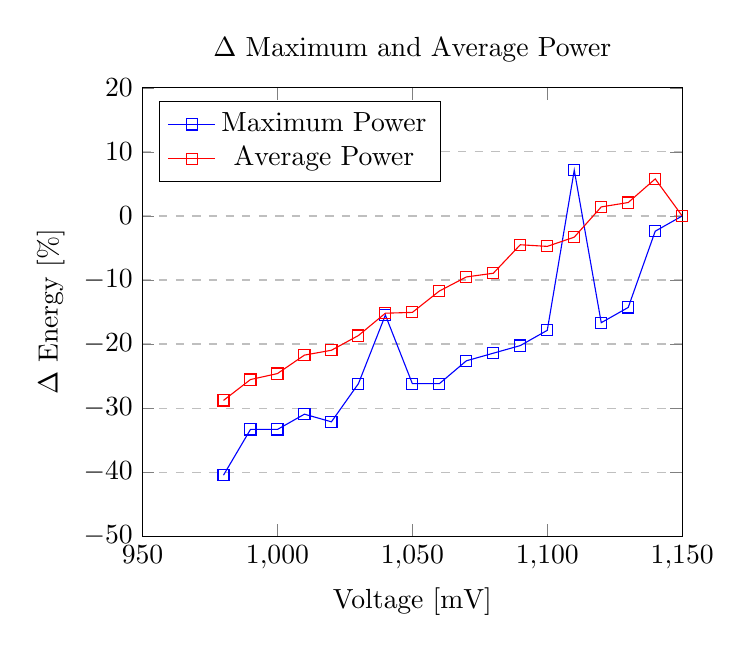
\begin{tikzpicture}
    \begin{axis}[
        title={$\Delta$ Maximum and Average Power},
        xlabel={Voltage [mV]},
        ylabel={$\Delta$ Energy [\%]},
        xmin=950, xmax=1150,
        ymin=-50, ymax=20,
        xtick={950,1000,1050,1100,1150,1200},
        ytick={-50,-40,-30,-20,-10,0,10,20},
        legend pos=north west,
        ymajorgrids=true,
        grid style=dashed,
    ]
     
    \addplot[
        color=blue,
        mark=square,
        ]
        coordinates {
        (1150, 0)
        (1140, -2.380952381)
        (1130, -14.28571429)
        (1120, -16.66666667)
        (1110, 7.142857143)
        (1100, -17.85714286)
        (1090, -20.23809524)
        (1080, -21.42857143)
        (1070, -22.61904762)
        (1060, -26.19047619)
        (1050, -26.19047619)
        (1040, -15.47619048)
        (1030, -26.19047619)
        (1020, -32.14285714)
        (1010, -30.95238095)
        (1000, -33.33333333)
        (990,  -33.33333333)
        (980,  -40.47619048)
        };
        \addlegendentry{Maximum Power}
    
    \addplot[
        color=red,
        mark=square,
        ]
        coordinates {
        (1150, 0)
        (1140, 5.785750379)
        (1130, 2.097018696)
        (1120, 1.414855988)
        (1110, -3.3097524)
        (1100, -4.749873674)
        (1090, -4.497220819)
        (1080, -8.943911066)
        (1070, -9.525012633)
        (1060, -11.72309247)
        (1050, -15.05811016)
        (1040, -15.18443658)
        (1030, -18.67104598)
        (1020, -20.97018696)
        (1010, -21.72814553)
        (1000, -24.60838807)
        (990,  -25.54320364)
        (980,  -28.80242547)
        };
        \addlegendentry{Average Power}
     
    \end{axis}
    \end{tikzpicture}
    \end{minipage}\hfill
    \begin{minipage}{.49\textwidth}
    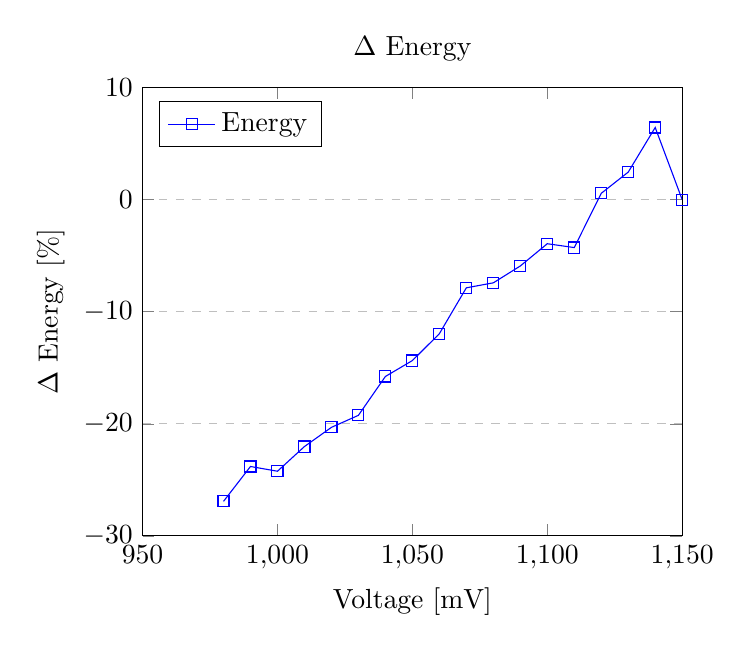
\begin{tikzpicture}
    \begin{axis}[
        title={$\Delta$ Energy},
        xlabel={Voltage [mV]},
        ylabel={$\Delta$ Energy [\%]},
        xmin=950, xmax=1150,
        ymin=-30, ymax=10,
        xtick={950,1000,1050,1100,1150,1200},
        ytick={-30,-20,-10,0,10},
        legend pos=north west,
        ymajorgrids=true,
        grid style=dashed,
    ]
     
    \addplot[
        color=blue,
        mark=square,
        ]
        coordinates {
        (980, -26.92226994)
        (990, -23.80800659)
        (1000, -24.23118962)
        (1010, -22.02895897)
        (1020, -20.31734614)
        (1030, -19.24458686)
        (1040, -15.77694737)
        (1050, -14.35819968)
        (1060, -11.963407)
        (1070, -7.86673507)
        (1080, -7.422421768)
        (1090, -5.919590672)
        (1100, -3.933564482)
        (1110, -4.275036236)
        (1120, 0.564039806)
        (1130, 2.456905505)
        (1140, 6.437273439)
        (1150, 0)
        };
        \legend{Energy}
     
    \end{axis}
    \end{tikzpicture}
    \end{minipage}
    \caption{Undervoltage on performance level 6.}
    \label{fig:under6}
\end{figure}

The subsequent inference runs using the default DVFS parameters always led to correct results, on all performance levels, which means that the trained weights achieved with non-conventional DVFS parameters can still be used to perform inference on another GPU running default parameters.

\begin{table}[!htb]
\centering
\begin{tabular}{l|llllllll}
\textbf{Performance Level}  & 0   & 1   & 2   & 3   & 4   & 5   & 6   & 7    \\
\textbf{Minimum Voltage [mV]}    & 800 & 800 & 840 & 880 & 910 & 940 & 980 & 1040 \\
\textbf{Undervolt {[}mV{]}} & 0   & 100 & 110 & 120 & 140 & 160 & 170 & 160 
\end{tabular}
\caption{Undervoltage Results}
\label{tab:undervoltage-res}
\end{table}

Hence, the achieved results show that there are benefits of finding the lowest voltage level since the power and energy reduction are substantial. Table \ref{tab:undervoltage-res} shows the amount of undervoltage that is possible to achieve for this CNN on each performance level. It is on the performance level 6 that more undervoltage capabilities are possible..



\subsubsection{Analysis}
The evidence that the performance of the application does decrease substantially with the increase in the core frequency/voltage may indicate that this type of application is overall memory bounded. However, it is necessary to explore the impacts of memory scaling further to confirm this theory. 

Nevertheless, even though the application, as a whole, may be memory bounded, some of the layers that construct the neural network may have different behaviour. A specific layer tunning mechanism may lead to both further reductions in energy consumption and performance increase.